\documentclass[a4paper]{jarticle}
%%% 本大会論文集固有のパラメータ,定義を読み込み.
    \usepackage{vrsjj}
%%% 図貼り付け用.必要に応じて,使用環境に適合するよう編集してください.
\usepackage[dvipdfmx]{graphicx}
%%% 最終ページの高さを自動的に揃える場合,balanceパッケージを使用可.
%%% multicolパッケージを使うと脚注が二段組でなくなるため,
%%% 脚注の仕組みを利用している英文著者の表示と干渉します.
\usepackage{balance}

\special{pdf: pagesize width 210truemm height 297truemm} 

%%% ヘッダ用定義.
\newcounter{vrsjyear}
\newcounter{vrsjmonth}
\newcounter{vrsjnum}

\setcounter{vrsjyear}{2025}
\setcounter{vrsjmonth}{9}
\setcounter{vrsjnum}{\value{vrsjyear}}
\addtocounter{vrsjnum}{-1995}

%%% 行間の指定: \baselinestrechの値が1.32で1ページ50行に相当します.
\renewcommand{\baselinestretch}{1.32}

\graphicspath{{./}} % 画像を置いておくフォルダ名

\begin{document}
\small %%% フォントのサイズを small (9 pt) に設定.
\twocolumn[%%%%%%%%%%%%%%%%%%%% []内が1段組部分.
%%%【必須】
\HeadComm{This article is a technical report without peer review, and its polished and/or extended version may be published elsewhere.}%
%%% 【必須】ロゴとヘッダ.変更しないでください.
\ProcTitle{第\arabic{vrsjnum}回日本バーチャルリアリティ学会大会論文集(\arabic{vrsjyear}年\arabic{vrsjmonth}月)}%
%%%
% 必須: 和文タイトル
\JTitle{VRコンテンツ体験時における生体・行動情報の統合に基づく\\リアルタイム感情推定フレームワーク}
% オプション: 英文タイトル
\ETitle{A Real-Time Emotion Estimation Framework Based on Integration of Physiological and Behavioral Information During VR Content Experience}
% 必須: 和文著者
\JAuthor{趙 聖化$^{1)}$}
% オプション: 英文著者
\EAuthor{Seika CHO}
% 必須: 和文所属
\Affiliation{1) 人間システム工学科 井村研究室}
% 必須: 和文要旨
\Abstract{本研究では,視線追跡機能付きHMDと複数の生体センサを統合し,VR体験中のユーザ感情をリアルタイムで推定するフレームワークを提案する.システム構成,データ処理,予備実験計画について述べる.}
% 必須: キーワード
\KeyWords{VR, 感情推定, 生体信号, 行動情報}
]

% ----- 図1(flowchart)のブロックを削除しました -----
% \begin{figure}[tp]
%  \centering
%  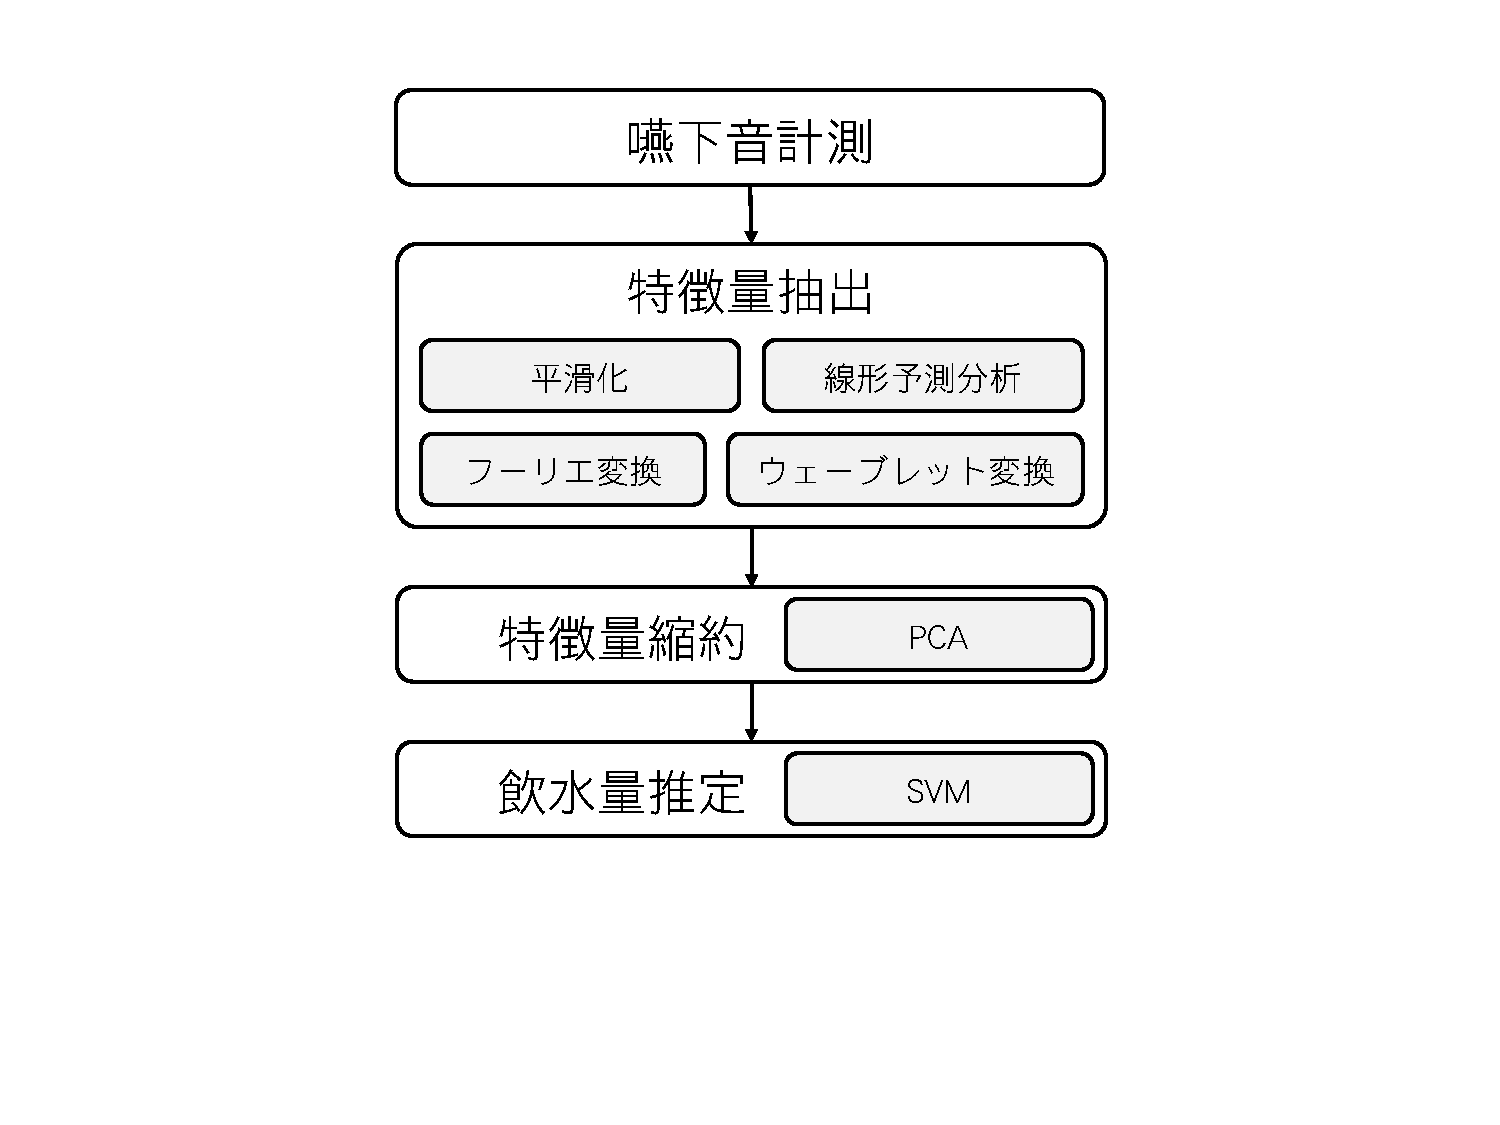
\includegraphics[width=\columnwidth]{flowchart.pdf}
%  \caption{提案する感情推定システムの処理フロー}
%  \label{fig:flow}
% \end{figure}

\section{はじめに}

VRコンテンツの評価は主観的であることが多く,制作者の意図した感情がユーザに伝わっているか客観的に把握することは難しい.本研究では,視線追跡機能付きHMD(ヘッドマウントディスプレイ),皮膚電気活動(EDA)・心電(ECG)・筋電(EMG)等の複数の生体センサを統合し,VRコンテンツ体験中のユーザの集中,恐怖,驚きといった感情を実時間で推定するフレームワークを構築する.

\section{関連研究}

生体信号を用いた感情推定は広く研究されている.EDAは情動的な覚醒度の指標として, 心拍変動(HRV)はストレスや感情の正負(valence)の評価に用いられている. 複数の生体信号を組み合わせることで,単一のセンサよりも高精度な感情推定が期待できる\cite{Guixeres2020, Glancy2021}.

VR環境下で生体信号を計測し,機械学習を用いて感情を分類する試みも活発になされている.Marín-Moralesら\cite{Marin-Morales2018}はEEG(Electroencephalogram)とHRV(Heart Rate Variability)からSVM(Support Vector Machine)を用いて覚醒度と感情価を推定している. また, Orozco-Moraら\cite{Orozco-Mora2024}はVRゲーム中のストレスレベルに応じて難易度を動的に調整するシステム(DDA)を試作しており, プレイヤーの心拍数に基づいてゲーム内パラメータを変化させることで, 恐怖や興奮を適切なレベルに維持できることを示している.

\section{提案手法}

本研究では,HMDと複数の生体センサを連携させ,VRコンテンツ体験中のユーザの感情を実時間で解析するシステムを構築する.

\subsection{システム構成とデータ収集}

視線・瞳孔径情報を取得可能なHMDを中核とし,外部センサとしてEDA,ECG,EMGセンサを連携させる. 多角的データから恐怖による心拍・発汗の上昇,驚きによる瞬きや筋収縮,集中による画面の凝視等を捉える. 加えて,コントローラの加速度情報や驚愕反応時のボタン入力も行動指標として取得する. 客観データはVR内のイベントログと時刻同期させ,体験後の主観評価アンケートと照合する.

\subsection{データ処理とリアルタイム推定}

収集した各センサデータから,リアルタイムで特徴量を抽出する.具体的には,EDAのピーク数,HRV指標(RMSSD:連続する心拍間隔差分の二乗平均平方根,LF/HF比:低周波/高周波成分比),EMGの振幅,瞳孔径変化量,コントローラからの行動データなどである.これらの特徴量を入力とし,感情の次元モデルとして広く知られるラッセルの円環モデル\cite{Russell1980}を参考に設定した安静,警戒,恐怖・驚愕といった感情ラベルに,ランダムフォレストやSVM, LSTMなどの機械学習モデルを用いて分類する.

リアルタイム推定においては,各信号の時間的特性を考慮する. 例えば,心拍やEMGのような即時的な反応は1\textasciitilde2秒という短い時間窓で変化を捉え,EDAのような遅れて現れる反応は6\textasciitilde10秒という長めの時間窓でトレンドを見ることで,推定の安定性と応答速度の両立を図る.

\section{予備実験計画}

提案手法を検証するため,以下の予備実験を計画する.

\begin{itemize}
    \item \textbf{現在の進捗:} 各センサからのデータ収集パイプラインの構築とサンプルコンテンツの制作を進めており、現在は製作者自身を対象としてシステムの動作確認を兼ねたデータ収集中である.
    \item \textbf{目的:} 構築したシステムがVRホラーによる感情喚起を正しく捉えられるか確認し,特徴量と感情の関係性を予備的に検証する.
    \item \textbf{被験者:} 5\textasciitilde10名程度の若年層ボランティアを対象とする.
    \item \textbf{手順:} VRホラーコンテンツを体験してもらい,その間の生体・行動データを記録する.体験後,アンケートにてシーンごとの主観的な恐怖度・驚き度・集中度を評価してもらう.
    \item \textbf{分析:} 収集した生体・行動データと主観評価,およびイベントログとの相関を分析する.心拍数やEDAの急上昇,コントローラの動きなどを確認する.このデータを用いて,感情分類モデルの予備的な学習と評価を行う.
\end{itemize}

\section{まとめと今後の課題}

本稿では,VRコンテンツ体験時におけるユーザの感情を,複数の生体センサを用いて実時間で推定する研究フレームワークを提案した.

今後の課題として,まず提案システムの基盤構築と,予備実験の実施(2025年6\textasciitilde9月)を進める .予備実験の結果に基づき,特徴量や機械学習モデルを洗練させた後,本実験と詳細な分析を行う(2025年10\textasciitilde11月) .最終的には,本研究の成果を,ユーザの感情状態に応じてコンテンツが動的に変化する適応型VRシステムの実現に繋げることを目指す.

\begin{thebibliography}{10}

\bibitem{Guixeres2020}
J. Guixeres, et al., Emotion Recognition in Immersive Virtual Reality: From Statistics to Affective Computing, \textit{Frontiers in Psychology}, Vol. 11, Article 1157, 2020.
    
\bibitem{Marin-Morales2018}
J. Marín-Morales, et al., Affective Computing in VR Environments using EEG and Heart Rate Variability, \textit{Sensors}, Vol. 18, No. 10, Article 3306, 2018.
    
\bibitem{Orozco-Mora2024}
C.E. Orozco-Mora, et al., Dynamic Difficulty Adaptation Based on Stress Detection for a VR Video Game: A Pilot Study, \textit{Electronics}, Vol. 13, No. 12, Article 2324, 2024.
    
\bibitem{Glancy2021}
M. Glancy and C.S. Ang, VREED: Virtual Reality Emotion Recognition Dataset using Eye Tracking \& Physiological Measures, \textit{Proc. ACM IMWUT}, Vol. 5, No. 4, Article 178, pp. 1-20, 2021.

\bibitem{Ogawa2014}
小川健一, 杉本泰治, 視線計測によるストレス評価手法の検討, \textit{日本バーチャルリアリティ学会論文誌}, Vol. 19, No. 1, pp. 61-70, 2014. 

\bibitem{Russell1980}
J. A. Russell, A circumplex model of affect, \textit{Journal of Personality and Social Psychology}, Vol. 39, No. 6, pp. 1161-1178, 1980.

\end{thebibliography}

\end{document}